\documentclass[notitlepage,12pt,a4paper]{article}
\usepackage{fullpage}

\usepackage{titling}
\pretitle{\begin{center}\Huge\bfseries}
\posttitle{\par\end{center}\vskip 0.5em}
\preauthor{\begin{center}\Large\ttfamily}
\postauthor{\end{center}}
\predate{\par\large\centering\ttfamily}
\postdate{\par}

\usepackage{subcaption}
\usepackage{graphicx}
\DeclareCaptionFormat{custom}
{
    \textbf{\small #1#2}\textnormal{\footnotesize #3}
}
\captionsetup{format=custom}

\usepackage[square,numbers]{natbib}
\bibliographystyle{abbrvnat}

\usepackage{enumitem}
\setlist{nolistsep}

\usepackage[normalem]{ulem}
\usepackage[colorlinks,linkcolor=black,urlcolor=blue,citecolor=blue]{hyperref}
\usepackage{url}
\usepackage{amsmath}
\usepackage{amssymb}
\usepackage{mathtools}
\usepackage[spanish]{babel}

\usepackage{caption}
\DeclareCaptionType{equ}[][]

\renewcommand{\baselinestretch}{2}
\title{Equilibrio Hidrostático en el Sol}
\author{Ramón Caballero Villegas}
\date{26 de Mayo de 2022}
\begin{document}

\maketitle

\section{Introducción}

En la hidrodinámica se observa un fenómeno denominado como el \textit{equilibrio
hidrostático}. Un fluido que está en equilibrio hidrostático está sometido a un
balance de fuerzas: aquellas que actúan en la dirección interna al fluido, y
aquellas causadas por la presión del mismo fluido. Estas fuerzas actúan en
direcciones opuestas y en magnitudes equivalentes, por lo cual el fluido no
experimenta una aceleración en total. Este balance de fuerzas ocurre en varios
escenarios dentro de nuestro universo, desde las profundidades de los océanos de
la Tierra hasta en las estrellas como nuestro Sol y planetas como Júpiter. Para
una parcela dentro del fluido (que cumpla con la \textit{hipótesis del
continuo}) estas fuerzas están dadas por la ecuación
\ref{balanceFuerzas_basico}, cuyos vectores pueden ser más fácilmente
visualizados en la figura \ref{balanceFuerzas_imgCubo}. Partiendo de esta se
puede llegar a la ecuación diferencial del equilibrio hidrostático en la
ecuación \ref{balanceFuerzas_diferencial}.

\begin{equ}[!ht]
	\begin{equation} \label{balanceFuerzas_basico}
		\sum F = 0 = p_{inferior} - p_{superior} -\rho g \Delta z
	\end{equation}
	\caption{Suma de fuerzas en una parcela de un fluido en equilibrio
	hidrostático, donde \(p_{inferior}\) y \(p_{superior}\) representan la
	presión que experimenta la parcela de fluido debido al fluido empujando a la
	parcela hacia al exterior y la presión causada por el peso del fluido por
	encima de la parcela respectivamente, \(\rho\) es la densidad de la parcela,
	y \(\Delta z\) es la longitud de la parcela en la dirección de la gravedad.}
\end{equ}

\begin{equ}[!ht]
	\begin{equation} \label{balanceFuerzas_diferencial}
		\frac{\mathrm{d} p}{\mathrm{d} z} = - \rho g
	\end{equation}
	\caption{Forma diferencial de la ecuación del equilibrio hidrostático.}
\end{equ}

\begin{figure}[!ht]
	\centering
	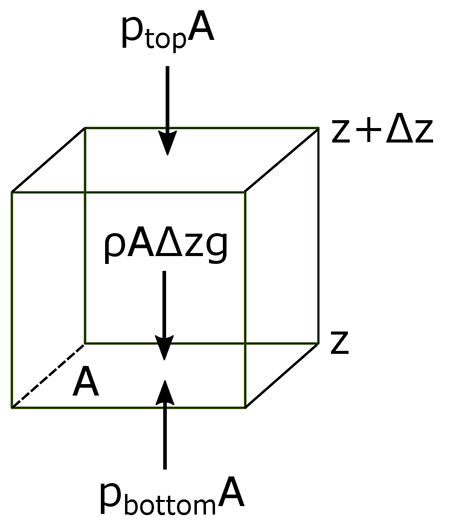
\includegraphics[scale=0.4]{Figuras/L2_hydrostatic_copy.png}
	\caption{Esquema representando las fuerzas en juego en una parcela de un
	fluido en equilibrio hidrostático considerando una forma cúbica de la
	parcela. Haciendo referencia a la ecuación \ref*{balanceFuerzas_basico},
	\(p_{bottom} = p_{inferior}\) y \(p_{top} = p_{superior}\).
	\cite{eqhsPennStateWebsite}}
	\label{balanceFuerzas_imgCubo}
\end{figure}

\subsection{Fluidos no Ideales}
Para que la ecuación \ref{balanceFuerzas_diferencial} pueda ser aplicada a un
problema particular requiere que la densidad \(\rho\) sea constante en el fluido
a lo largo del espacio y del tiempo, es decir requiere que el problema trate de
un \textit{fluido incompresible}. El plasma en el Sol no cumple con este
requisito; la densidad del plasma varía con la altitud en el Sol. La presión y
la temperatura también dependen de la altitud. En estas situaciones se debe
considerar una \textit{ecuación de estado}, la cual acopla estas variables
fluido entre si. La ecuación de gases ideales es un ejemplo de una ecuación de
estado: \(PV = nRT\), la cual incluye la presión y temperatura explícitamente y
la densidad de manera implícita (\(\rho = \frac{n}{V}\)). Sin embargo, esta
ecuación asume que la temperatura es constante con la altitud; para analizar el
equilibrio hidrostático en la superficie del Sol necesitaremos un modelo cuya
temperatura no sea constante en el espacio.

\subsection{Equilibrio Hidrostático Dentro del Sol}

\subsubsection{Modelo Analítico} \label{sec:modeloAnalitico}

Para el problema resuelto en este proyecto consideramos un modelo del Sol en
equilibrio hidrostático. El Sol está compuesto principalmente de hidrógeno
atómico, el cual funciona como el combustible principal para las reacciones
nucleares que ocurren en su núcleo. Estas reacciones generan la presión interna
que balancea el peso gravitacional del mismo Sol debido a su masa. La presión de
un plasma de hidrógeno ionizado se puede modelar usando la ecuación
\ref{ecEstadoPlasmaHidrogeno}. 

\begin{equ}[!ht]
	\begin{equation} \label{ecEstadoPlasmaHidrogeno}
		p(z) = \frac{2 k_B \rho (z) T(z)}{m_p}
	\end{equation}
	\caption{Ecuación de estado dentro del Sol. \(k_B\) es la constante de
	Boltzmann, \(\rho (z)\) es la densidad con respecto a la altitud, \(T(z)\)
	es la temperatura con respecto a la altitud, y \(m_p\) es la masa molecular
	promedio del fluido, que en el caso del Sol la tomamos como la masa del
	hidrógeno atómico. \cite{newtonianCafe}}
\end{equ}

Al integrar la ecuación \ref{balanceFuerzas_diferencial} sustituyendo la
ecuación \ref{ecEstadoPlasmaHidrogeno} como la ecuación de estado obtenemos el
siguiente modelo de la presión solar en la ecuación \ref{ecPresionNoIntegrada}.

\begin{equ}[!ht]
	\begin{equation} \label{ecPresionNoIntegrada}
		p(z) = p(z_0) \exp \left(- \frac{m_p g}{2 k_B} \int_{z_0}^{z} \frac{\mathrm{d} z}{T(z)}\right)
	\end{equation}
	\caption{Presión térmica del gas ionizado en la fotosfera del Sol.
	\(p(z_0)\) es la presión a la altitud de referencia, la cual para este
	problema se toma que \(z_0 = 0 \textrm{ Mm}\), la superficie de la
	fotosfera.}
\end{equ}

Para poder integrar la ecuación \ref{ecPresionNoIntegrada} correctamente se debe
considerar un perfil de temperatura dependiente de la altitud, para la cual se
utiliza la ecuación \ref{ecTemperaturaAnalitica}.

\begin{equ}[!ht]
	\begin{equation} \label{ecTemperaturaAnalitica}
		T(z) = \frac{1}{2} T_{cor} \left(1 + dtc + \left(1 - dtc\right) \tanh \left(\frac{z - z_t}{z_w}\right)\right)
	\end{equation}
	\caption{Perfil de temperatura en la fotosfera solar. Este está definido por
	varios constantes obtenidos del Sol: \(dtc = T_{phot} / T_{cor}\), donde
	\(T_{phot} = 6000 \textrm{ K}\) es la temperatura en la base de la fotosfera
	y \(T_{cor} = 1.2 \times 10^6 \textrm{ K}\) es la temperatura en la corona.
	La región de separación entre la fotosfera y la corona viene representada en
	\(z_t = 2 \textrm{ Mm}\) y \(z_w = 0.2 \textrm{ Mm}\), las cuales
	representan la altitud y el grosor de esta región de transición
	respectivamente. \cite{newtonianCafe}} 
\end{equ}

Dado este perfil de temperatura podemos integrar la ecuación
\ref{ecPresionNoIntegrada} para terminar con la ecuación
\ref{ecPresionIntegralAnalitica} integrada para la presión con respecto a la
altitud. Una vez integrada analíticamente se puede usar para encontrar la
presión en la atmósfera solar a una altitud \(z\); esto nos permitirá encontrar
la densidad del plasma usando la ecuación de estado, modificando la ecuación
\ref{ecEstadoPlasmaHidrogeno} para darnos la densidad del plasma, visto en la
ecuación \ref{ecEstadoDensidadAnalitico}.

\begin{equ}[!ht]
	\begin{equation} \label{ecPresionIntegralAnalitica}
		p(z) = p(z_0) \exp \left(
			- \frac{m_p g}{2 k_B} 
			\left(
				\frac{
					\left(dtc - 1\right) \cdot z_w \cdot
					\ln \left(
						dtc \cdot 
						\exp \left(
							\frac{2 z_t}{z_w} - \frac{2 z}{z_w}
						\right) + 1
					\right) 
				}{
					2 \cdot T_{cor} \cdot dtc
				}
				+ \frac{z}{T_{cor}}
			\right)
		\right)
	\end{equation}
	\caption{Ecuación de presión dependiente de la altitud, integrada usando el perfil de temperatura definido.}
\end{equ}

\begin{equ}[!ht]
	\begin{equation} \label{ecEstadoDensidadAnalitico}
		\rho (z) = \frac{m_p p(z)}{2 k_B T(z)}
	\end{equation}
	\caption{Ecuación de estado del plasma ionizado, presentada de una manera
	que facilita encontrar la densidad del plasma a una altitud \(z\) dado la
	presión y temperatura a esta altitud. \cite{newtonianCafe}}
\end{equ}

\subsubsection{Modelo C7} \label{sec:c7Modelo}
El modelo C7 describe el perfil de temperatura del Sol en su estado inactivo
promedio, enfocado en la cromosfera y la región de transición a la corona.
\cite{c7ModelPaper} Este modelo unidimensional e independiente del tiempo está
basado principalmente en observaciones hechas en el ultravioleta extremo. Este
perfil se puede visualizar en la figura \ref{c7TemperaturaGrafica}.

\begin{figure}[!ht]
	\centering
	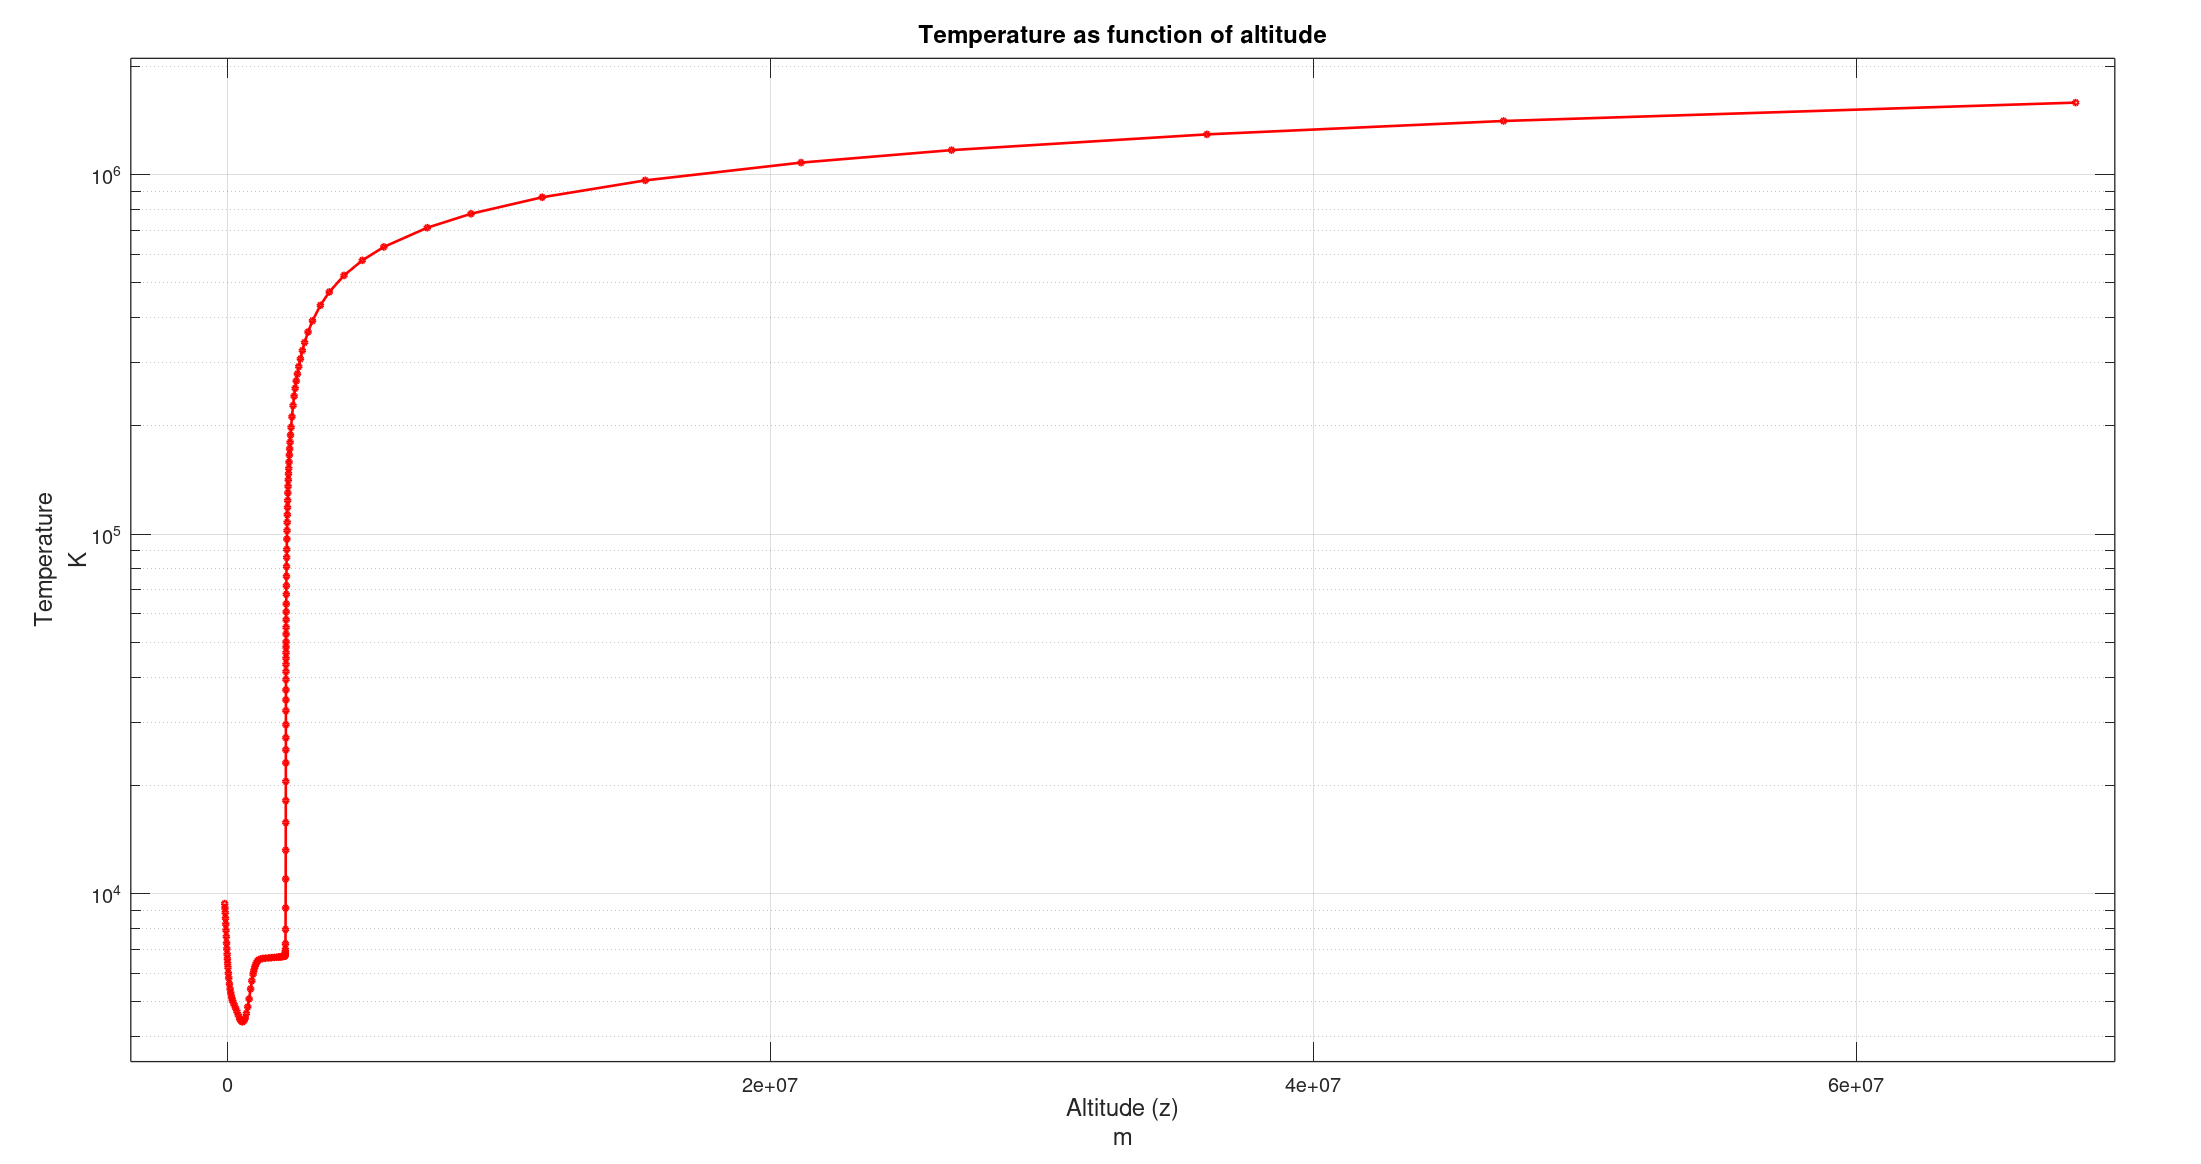
\includegraphics[scale=0.3]{Figuras/C7ModeloTemperaturaGrafica.png}
	\caption{Perfil de temperatura en la cromosfera del Sol, incluyendo la región de transición a la corona. Esta región de transición se puede ver en el fuerte empinamiento de la gráfica, donde la temperatura aumenta rápidamente a niveles mayores de lo visto en la cromosfera.}
	\label{c7TemperaturaGrafica}
\end{figure}

El perfil de temperatura visualizado en la figura \ref{c7TemperaturaGrafica} no
está definido de forma analítica como la ecuación \ref{ecTemperaturaAnalitica},
si no que es un conjunto de datos discretos, dándonos la temperatura en la
atmósfera del Sol a cierta altitud. Para obtener los perfiles de densidad y
presión del plasma en esta región se necesitan las ecuaciones \ref{ecPresionC7}
a \ref{ecScaleHeightC7}:

\begin{equ}[!ht]
	\begin{align}
		p_e (z) = p_{ref} \exp \left(- \int_{z_{ref}}^{z} \frac{dz}{\Lambda (z)}\right) \label{ecPresionC7} \\
		\rho_e (z) = \frac{p_e (z)}{g \Lambda (z)} \label{ecDensidadC7} \\
		\Lambda (z) = \frac{k_B T_e (z)}{m g} \label{ecScaleHeightC7}
	\end{align}
	\caption*{Ecuaciones del equilibrio hidrostático para el modelo C7 de
	temperatura. \cite{newtonianCafe} \(\Lambda (z)\) es la altura de escala, la
	cual modela el decrecimiento de la temperatura del plasma con respecto a la
	altitud.} 
\end{equ}

Debido a la ausencia de una solución analítica para estas ecuaciones, estas
deben ser resueltas usando un método numérico. A continuación explico los
códigos que se desarrollaron para resolver este problema.
\section{Códigos de Integración}

Para trabajar de una manera más eficiente se desarrollaron dos códigos separados
basado en su funcionalidad: unos scripts en Octave, la cual facilita operaciones
matemáticas y la creación de gráficas de una manera más declarativa, y un código
en C++, el cual ofrece mayor control sobre las instrucciones que debe correr el
programa y mayor extensibilidad. Los scripts de Octave fueron utilizados para
las soluciones analíticas para el modelo descrito en la sección
\ref{sec:modeloAnalitico}, mientras que el código de C++ fue utilizado para el
modelo C7 (sección \ref{sec:c7Modelo}). Ambas soluciones fueron graficadas
usando los scripts de Octave. El código completo se puede encontrar y descargar
del repositorio de GitHub
\href{https://github.com/KnightIV/EquilibrioHidrostatico}{EquilibrioHidrostatico}.

\subsection{Solución Analítica}

\subsubsection{Implementación del Código}
Las soluciones para el modelo analítico del equilibrio hidrostático en la
fotosfera del Sol están implementadas en el archivo
\verb|Graficas_EcuacionIdeal.m|. Aquí se definen las ecuaciones descritas la
sección \ref{sec:modeloAnalitico} dependientes de la altitud, representada por
el arreglo \verb|z| de \verb|6000| entradas, representando las altitudes en
metros para las cuales se van a resolver las ecuaciones. Este arreglo está
declarado en la parte superior del código junto al resto de las constantes
físicas necesarias para resolver el problema. 

Estas soluciones no pueden ser generadas todas al mismo tiempo debido a su
acoplamiento entre si, por lo que fue necesario resolverlas en un orden
específico. Para encontrar la densidad con respecto a la altitud se necesita
saber la presión; la presión requiere la integral del perfil de temperatura. Una
vez que cada una haya sido calculada se puede incluir en la subsecuente
ecuación. Debido que el propósito principal de Octave es facilitar la evaluación
de expresiones matemáticas estas operaciones son implementadas de manera
declarativa, cuya notación no es muy diferente que su representación matemática. 

\subsubsection{Resultados}
Una vez terminado el cálculo de cada ecuación el mismo script se encarga de
graficar los resultados. Esto se hace por conveniencia, ya que los datos siguen
en la memoria del programa corriendo. Para hacer esta parte más modular se
separó la función de graficar a un archivo separado dentro del proyecto, llamado
igual que la función \verb|plot_data_helper.m|. Aparte de separar la lógica del
código, esto también permite usar esta subrutina en el script que acompaña la
solución numérica. Los perfiles de presión, temperatura, y densidad obtenidos
mediante una integración analítica se pueden ver en la figura
\ref{modeloAnaliticoResultadosGraficas}, en las cuales se puede observar el
perfil suave que tienen cada una de las funciones. 

\begin{figure}[!ht]
	\centering
	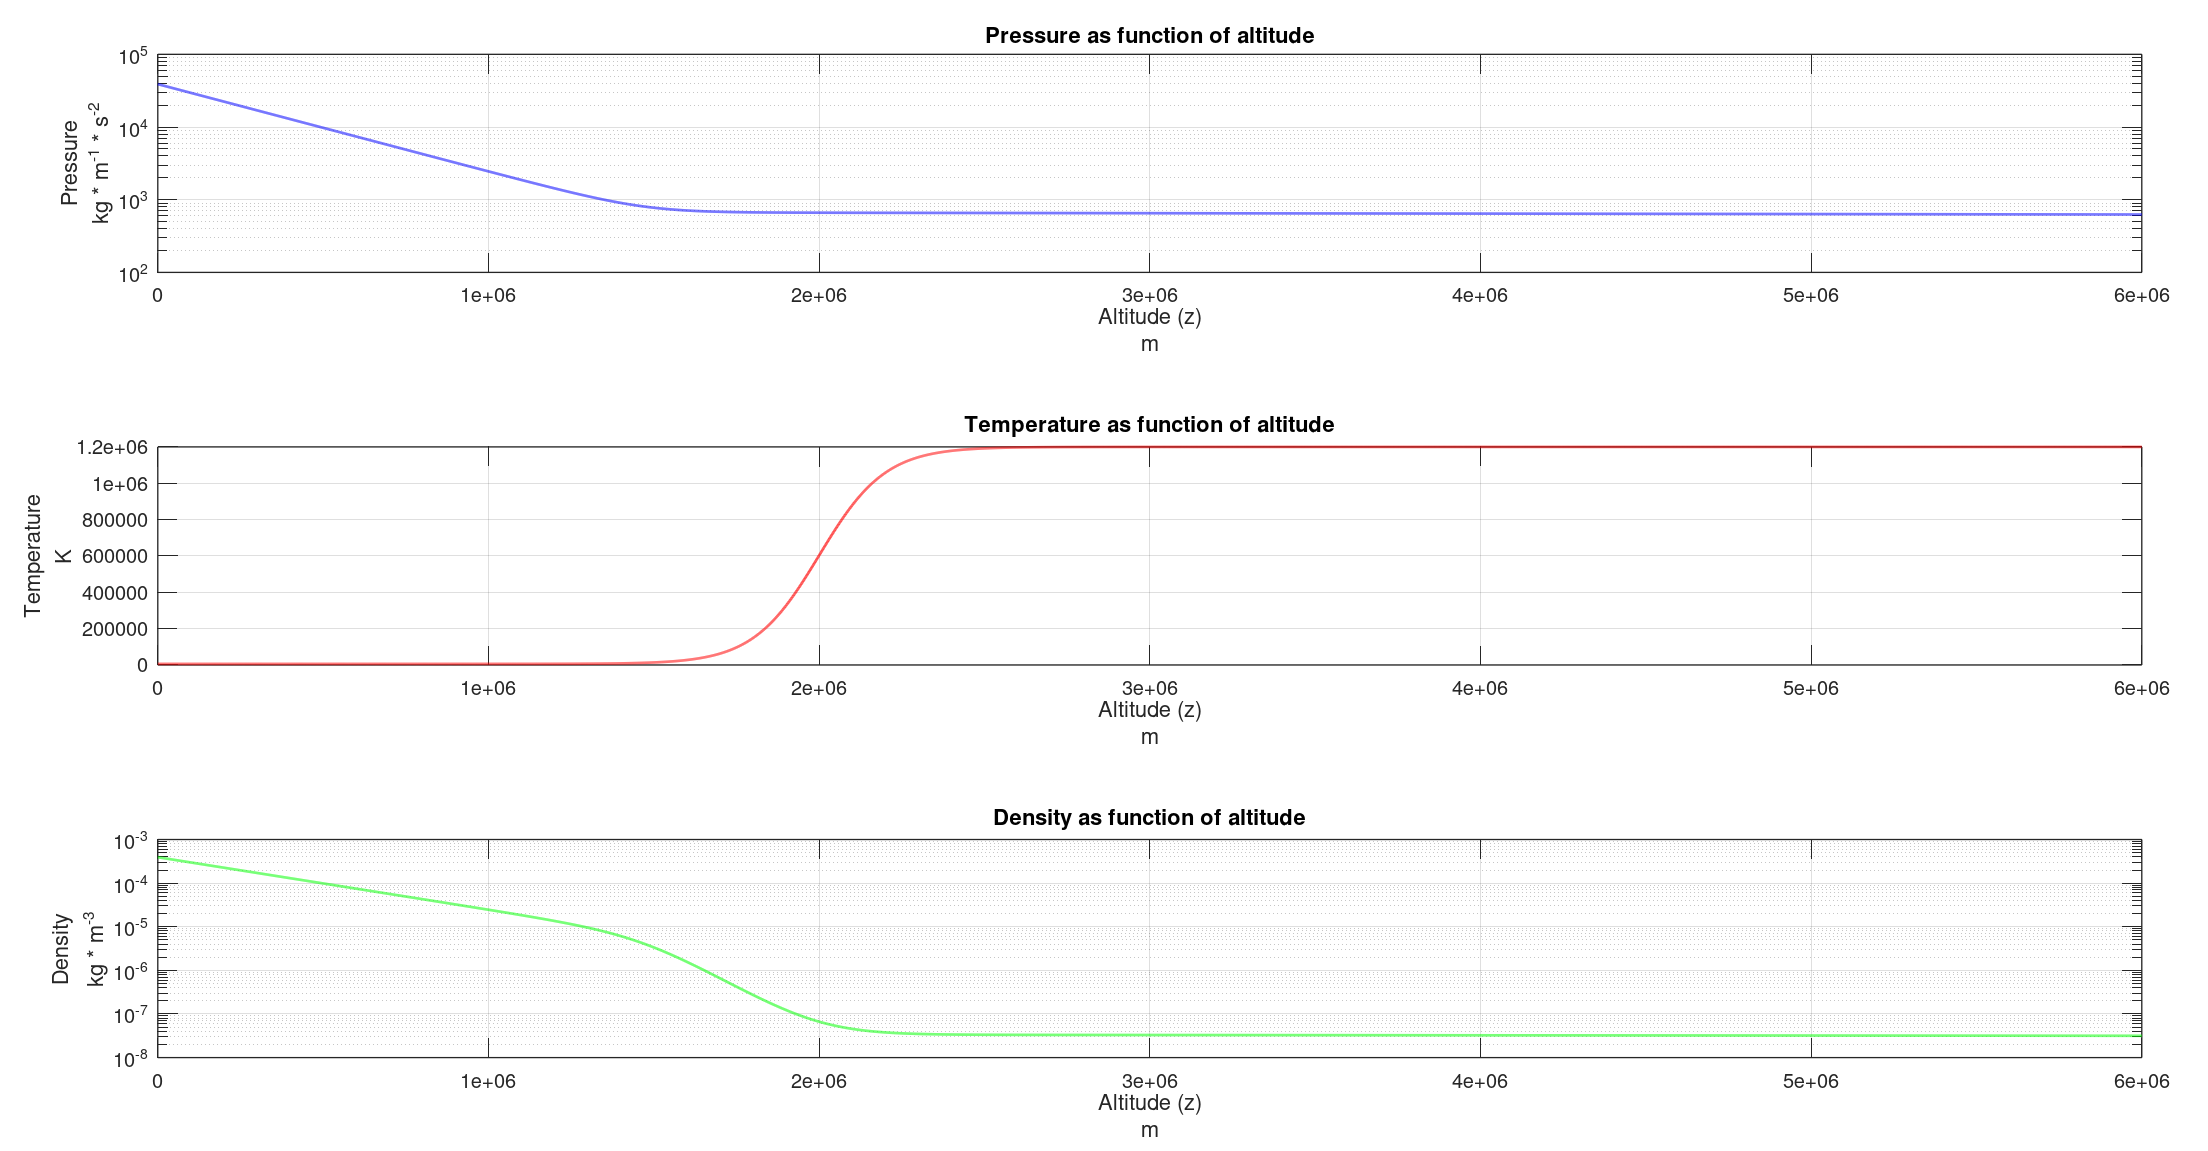
\includegraphics[scale=0.3]{Figuras/IntegracionAnaliticaGrafica.png}
	\caption{Perfiles de presión, temperatura, y densidad del plasma en la fotosfera y la región de transición a la corona.}
	\label{modeloAnaliticoResultadosGraficas}
\end{figure}

\subsection{Solución Numérica del Modelo C7}

\subsubsection{Implementación del Código}
A diferencia del código utilizado para la integración de las ecuaciones
analíticas, el modelo C7 fue resuelto con un código en C++. Este lenguaje fue
seleccionado por varias razones:

\begin{itemize}
	\item Habilidad de programar módulos por separado, incluyendo compilación.
	Esta fue la razón principal por la cual está escrita en C++, dejando abierta
	la posibilidad de implementar el código de integración numérica para que sea
	ejecutable en un procesador de gráficos (GPU). 
	\item Mayor control sobre las operaciones implementadas.
 	\item Compatibilidad entre Windows y Linux sin necesitar de varias
 	dependencias, con la excepción de herramientas de compilación.
\end{itemize}

El proyecto en si consiste de dos sub-proyectos, cada uno responsable de
diferentes funciones. El proyecto ejecutable, \verb|EquilibrioHidrostatico|,
contiene la rutina principal (la función \verb|main| requerida en todo
ejecutable escrito en C++) del programa, la cual hace llamadas a los módulos de
integración y extracción de datos descritos en las siguientes secciones. Este
código también cuenta con funcionalidad para medir el tiempo de ejecución, para
medir correctamente la eficiencia del programa en cuanto al tiempo.

Una de las características principales de este código es que todos los datos los
mantiene en su memoria durante la ejecución del programa, en vez de calcular los
valores necesarios para cada altitud y escribir estos a un archivo
inmediatamente. A pesar de que esto sería lo más eficiente en cuanto al uso de
memoria del programa, esto le agregaría complejidad al programa, a diferencia de
mantener los datos en la memoria en todo momento. A pesar de esto, midiendo la
cantidad de memoria consumida por el programa al final de su ejecución revela
que solo ocupa 713 kB de memoria, la mayoría siendo la consecuencia de escribir
los resultados al archivo. El resto del código hace uso de punteros de memoria,
usando la estructura \verb|shared_ptr| para evitar la complejidad que resultaría
al tener que manejar los punteros de manera manual. Gracias a estos los datos
numéricos solo son almacenados una vez durante todo el programa sin necesidad de
crear copias de los arreglos, evitando el malgasto de memoria.

\subsubsection{\texttt{EQHS\textunderscore Data}} \label{sec:eqhsData} Este
módulo contiene subrutinas que facilitan la interacción con los datos numéricos
de la simulación. En particular vienen dos funciones importantes:
\verb|get_alt_temp_values| y \verb|export_data_csv| que se encargan de leer los
datos del perfil de temperaturas y exportar los resultados respectivamente. 

Para empezar a resolver las ecuaciones definidas en la sección
\ref{sec:c7Modelo} el código lee los datos de temperatura dados en el archivo
\verb|Temperature-C7.dat| dentro del sub-proyecto \verb|EQHS_Data|. En total
estos vienen siendo en total 140 puntos de datos a varios niveles de altitud. En
estos definimos la altitud 0 como el nivel de referencia, el cual se va a
utilizar durante la integración numérica. Estos datos son almacenados dentro del
programa en arreglos separados para facilitar los cálculos en las subsecuentes
subrutinas. La función \verb|get_alt_temp_values| es la primera invocada en el
programa.

Una vez resuelto las ecuaciones del modelo C7 se pueden exportar en formato CSV
para facilitar su lectura en programas externos (incluyendo el script en Octave
que se usará para graficar los datos finales) usando la subrutina
\verb|export_data_csv|. La función crea la carpeta y el archivo de resultados en
el caso de no existir, y simplemente escribe los resultados en una tabla en el
archivo, la cual es fácilmente legible por humanos y programas de computadoras.

\subsubsection{\texttt{EQHS\textunderscore Integrador}} El módulo integrador
consiste de una función responsable por la integración numérica y una clase que
encapsula los datos correspondientes a las funciones del plasma solar. A
continuación viene una breve explicación de la funcionalidad expuesta
públicamente a los proyectos dependiente del \verb|EQHS_Integrador|.

Para facilitar el acoplamiento de datos en el código (particularmente entre la
altitud y las varias propiedades del plasma como su temperatura y densidad) este
módulo integrador define una clase contenedor de datos en \verb|DataContainer.h|
llamado \verb|AltitudeFunction|. Instancias de esta clase no hacen nada más que
envolver los datos numéricos en una forma conveniente con cual trabajar sin
crear copias innecesarias de los arreglos. 

Dentro de \verb|Integrador.h| viene definido una única función que hace la
integración numérica y regresa como resultado las funciones de altura de escala,
presión, y densidad con respecto a la altitud en forma de varias instancias de
la clase \verb|AltitudeFunction|. La integración numérica de la escala de
altura, tal como la requiere la ecuación \ref{ecPresionC7}, se lleva a cabo
mediante una regla de trapecio a lo largo de la temperatura. Esto nos permite
tener una alta eficiencia en la integración, siendo que el algoritmo crece
linealmente con el tamaño del arreglo de temperatura dados por el archivo de
datos. Una vez que los resultados hayan sido generados se pueden regresar al
programa principal para poder exportar tal como se mencionó en la sección
previa.

\subsubsection{Resultados}
Al terminar la integración numérica y tener todos los resultados guardados en la
memoria del programa el último paso es exportar los datos tal como fue
mencionado en la sección \ref{sec:eqhsData}. Las gráficas en la figura
\ref{modeloNumericoResultadosGraficas} fueron generadas usando Octave, con el
script \verb|Graficas_EquilibrioHidrostaticoPerfil.m|. 

\begin{figure}[!ht]
	\centering
	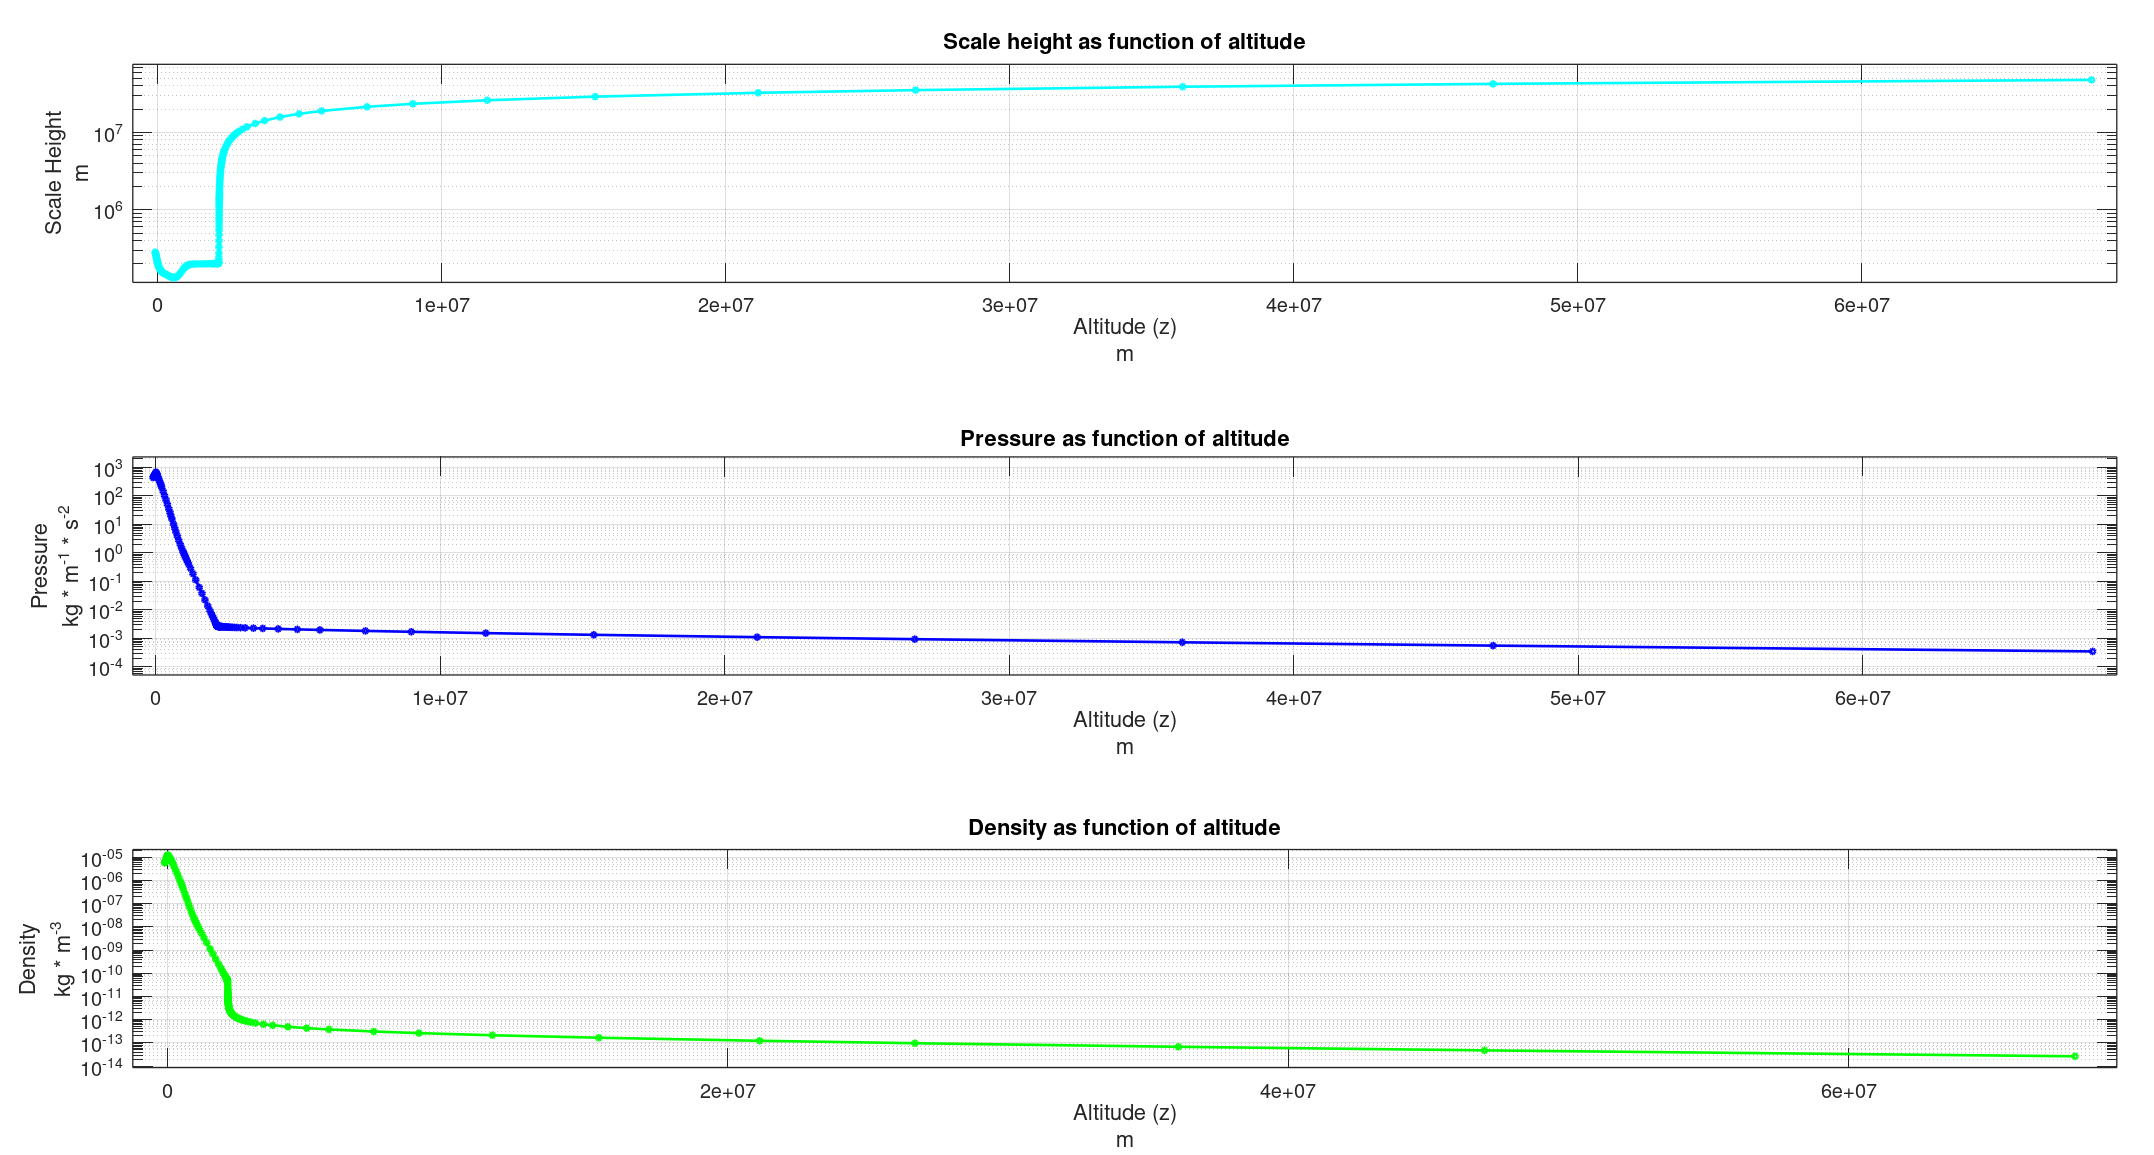
\includegraphics[scale=0.3]{Figuras/IntegracionNumericaGrafica.png}
	\caption{Perfiles de altura de escala, presión, y densidad del plasma en la
	fotosfera y la región de transición a la corona. En estas figuras los puntos
	sólidos representan los valores obtenidos de la integración numérica, de los
	cuales Octave puede interpolar para generar una función suave. Se puede
	observar que la altura de escala tiene el mismo perfil que la temperatura
	del modelo C7 visto en la figura \ref{c7TemperaturaGrafica}. Se puede ver la
	región de transición entre la cromosfera y la corona en las regiones de
	decaimiento rápido de la presión y la densidad, mientras que la temperatura
	(y como consecuencia, la altura de escala) experimenta un aumento brusco.}
	\label{modeloNumericoResultadosGraficas}
\end{figure}

\clearpage
\bibliography{ref}
\end{document}